% !TeX root = ../thuthesis-example.tex

\chapter{PLATFORM DEVELOPMENT}

Several challenges were faced during the development:
\begin{enumerate}
    \item Distribution of the source code;
    \item Distribution of the NUIX-Studio App demos;
    \item Creating Tutorials;
    \item Providing API for external projects;
    \item Updating the dependencies;
    \item Rewriting the code to support new architectures.
\end{enumerate}

The platform's source code is hosted at \cite{NUIXStudio} repository. The source code distribution required keeping the repository size at a minimum while providing an easy installation procedure. NUIX-Studio was shared as a separate package to follow these requirements.

The NUIX-Studio platform prototypes did not initially support Virtual reality (Figure~\ref{fig:Prototype2-figure}).


\begin{figure}
  \centering
  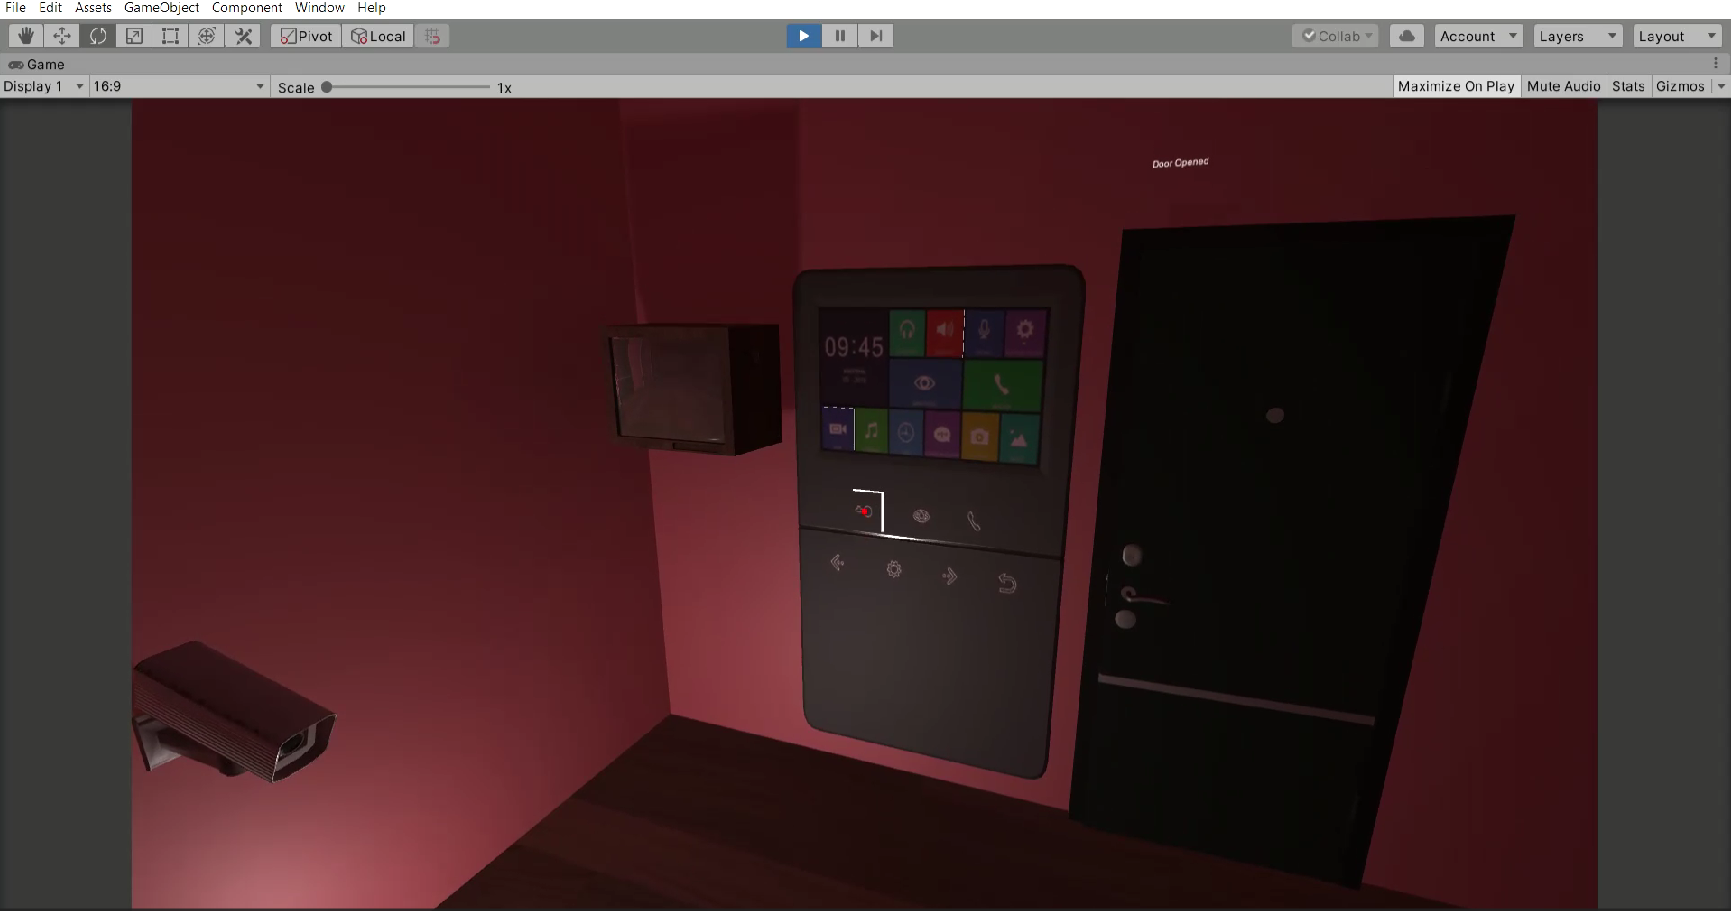
\includegraphics[width=0.6\linewidth]{figures/Prototype2.png}
  \caption{The second prototype of the VR-IoT Research platform}
  \label{fig:Prototype2-figure}
\end{figure}

The final structure used in NUIX-Studio is different from the structure in Figure~\ref{fig:Prototype3Structure-figure}. The server was responsible for storing and synchronizing item parameters and keeping all the Unity-specific functionality in the previous prototypes. The Unity Integration package job was to create Item representations for Virtual reality and share them to other NUIX-Studio App instances as Unity objects. This approach's main limitation is that Unity objects have a much bigger size than the Data Transfer Objects (DTO) used in the final prototype. These Unity objects were synchronized every frame for the simultaneous work, which dramatically dropped the NUIX-Studio App instances' performance and made the solution not scalable.

\begin{figure}
  \centering
  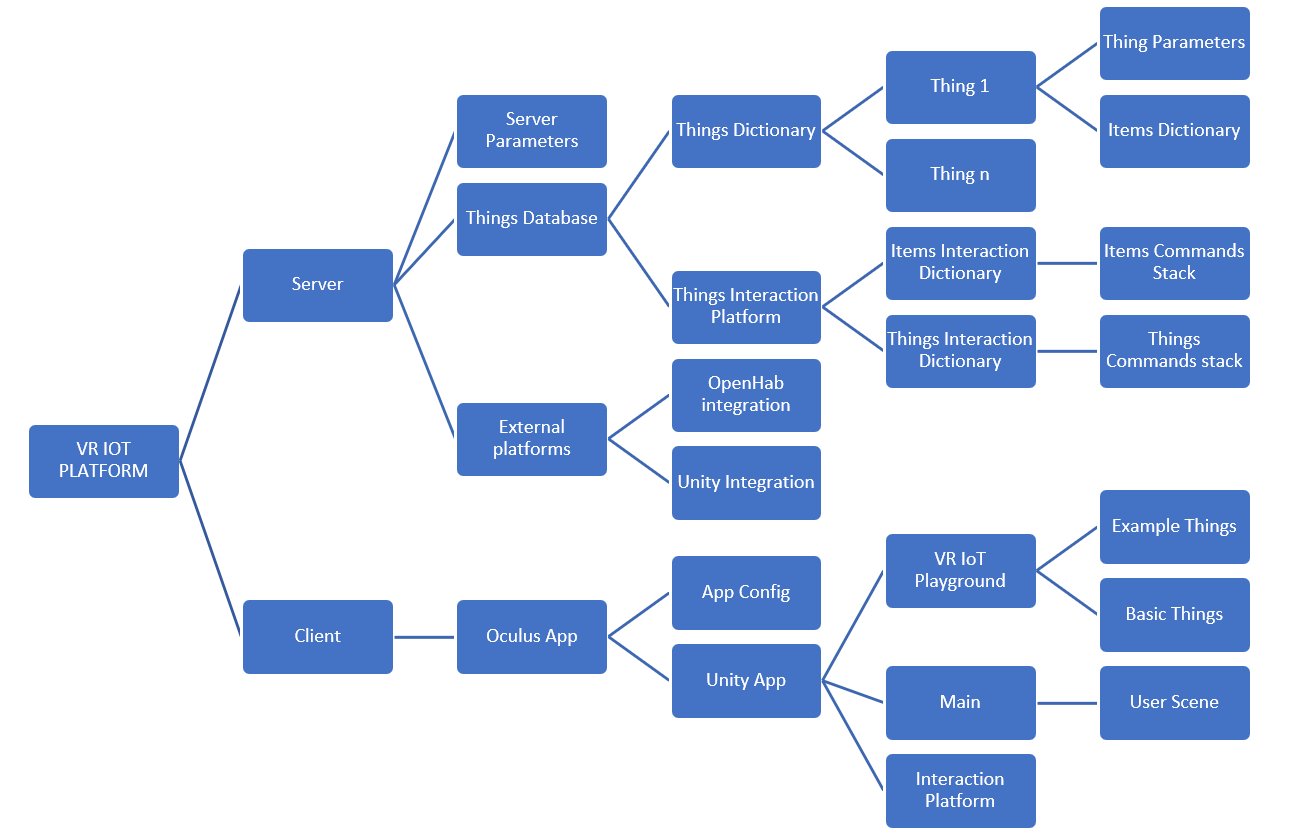
\includegraphics[width=0.9\linewidth]{figures/Prototype3Structure.png}
  \caption{The third prototype's structure}
  \label{fig:Prototype3Structure-figure}
\end{figure}

The third prototype provided only a button Widget (Figure~\ref{fig:Prototype3-figure}), but after integrating Mixed Reality Toolkit into the fourth prototype (Figure~\ref{fig:Prototype4-figure}), additional Widgets were added to the platform. 

\begin{figure}
  \centering
  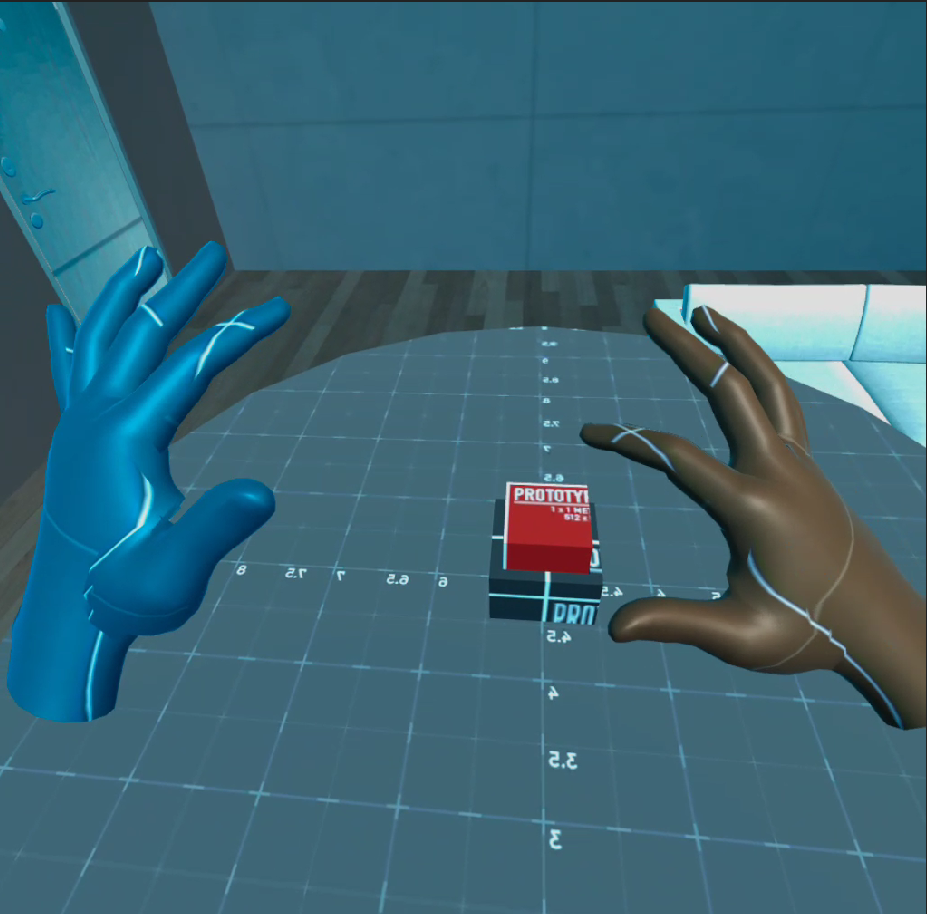
\includegraphics[width=0.6\linewidth]{figures/Prototype3.png}
  \caption{The third prototype of the VR-IoT Research platform. Button Widget.}
  \label{fig:Prototype3-figure}
\end{figure}

\begin{figure}
  \centering
  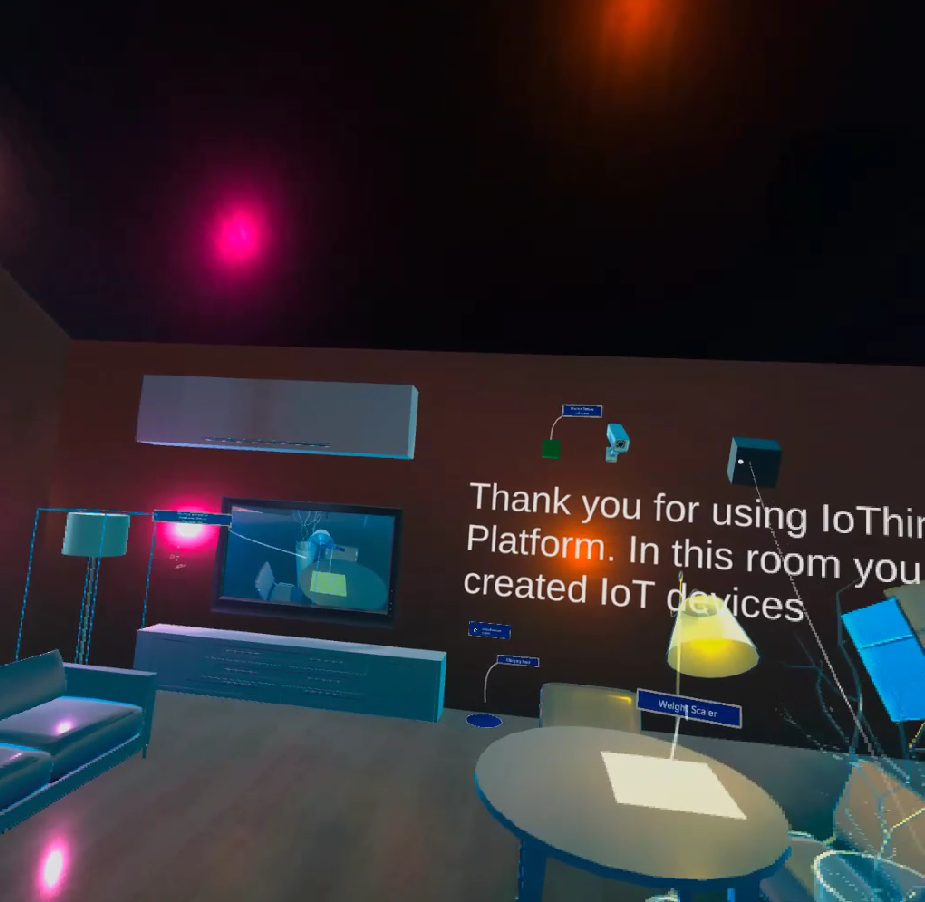
\includegraphics[width=0.6\linewidth]{figures/Prototype4.png}
  \caption{The fourth prototype of the VR-IoT Research platform. A virtual copy of the real-world Smart home environment was used with virtual items added, such as location, contact, player, switch, and dimmer items. Also several Widgets were supported: sight sensor, motor, light widget, pressure sensor, video streaming screens and gesture recognition.}
  \label{fig:Prototype4-figure}
\end{figure}

Another important feature added in the fourth prototype was the Input Simulation Service (Figure~\ref{fig:InputSimulation-figure}). Previously, in most cases, testing the interaction with Widgets required using a Virtual reality Headset. To use an Oculus Quest VR Headset, developers need to prepare their workplace. Firstly, it is necessary that the environment for using the Virtual reality Headset is well lit, otherwise, the detection of the position of Virtual reality Headset in the world space will not work correctly. Secondly, a sufficient amount of space around the developer is needed to be able to move the Virtual reality Headset controllers or hands freely. Unfortunately, these requirements for setting up the environment are often infeasible. With the help of the Input Simulation Service system, based on the Mixed Reality Toolkit, it became possible not only to move inside the virtual world but also to make movements with virtual hands, including the various gestures simulation.

\begin{figure}
  \centering
  \subcaptionbox{Pinching gesture simulation\label{fig:InputSimulation-a}}
    {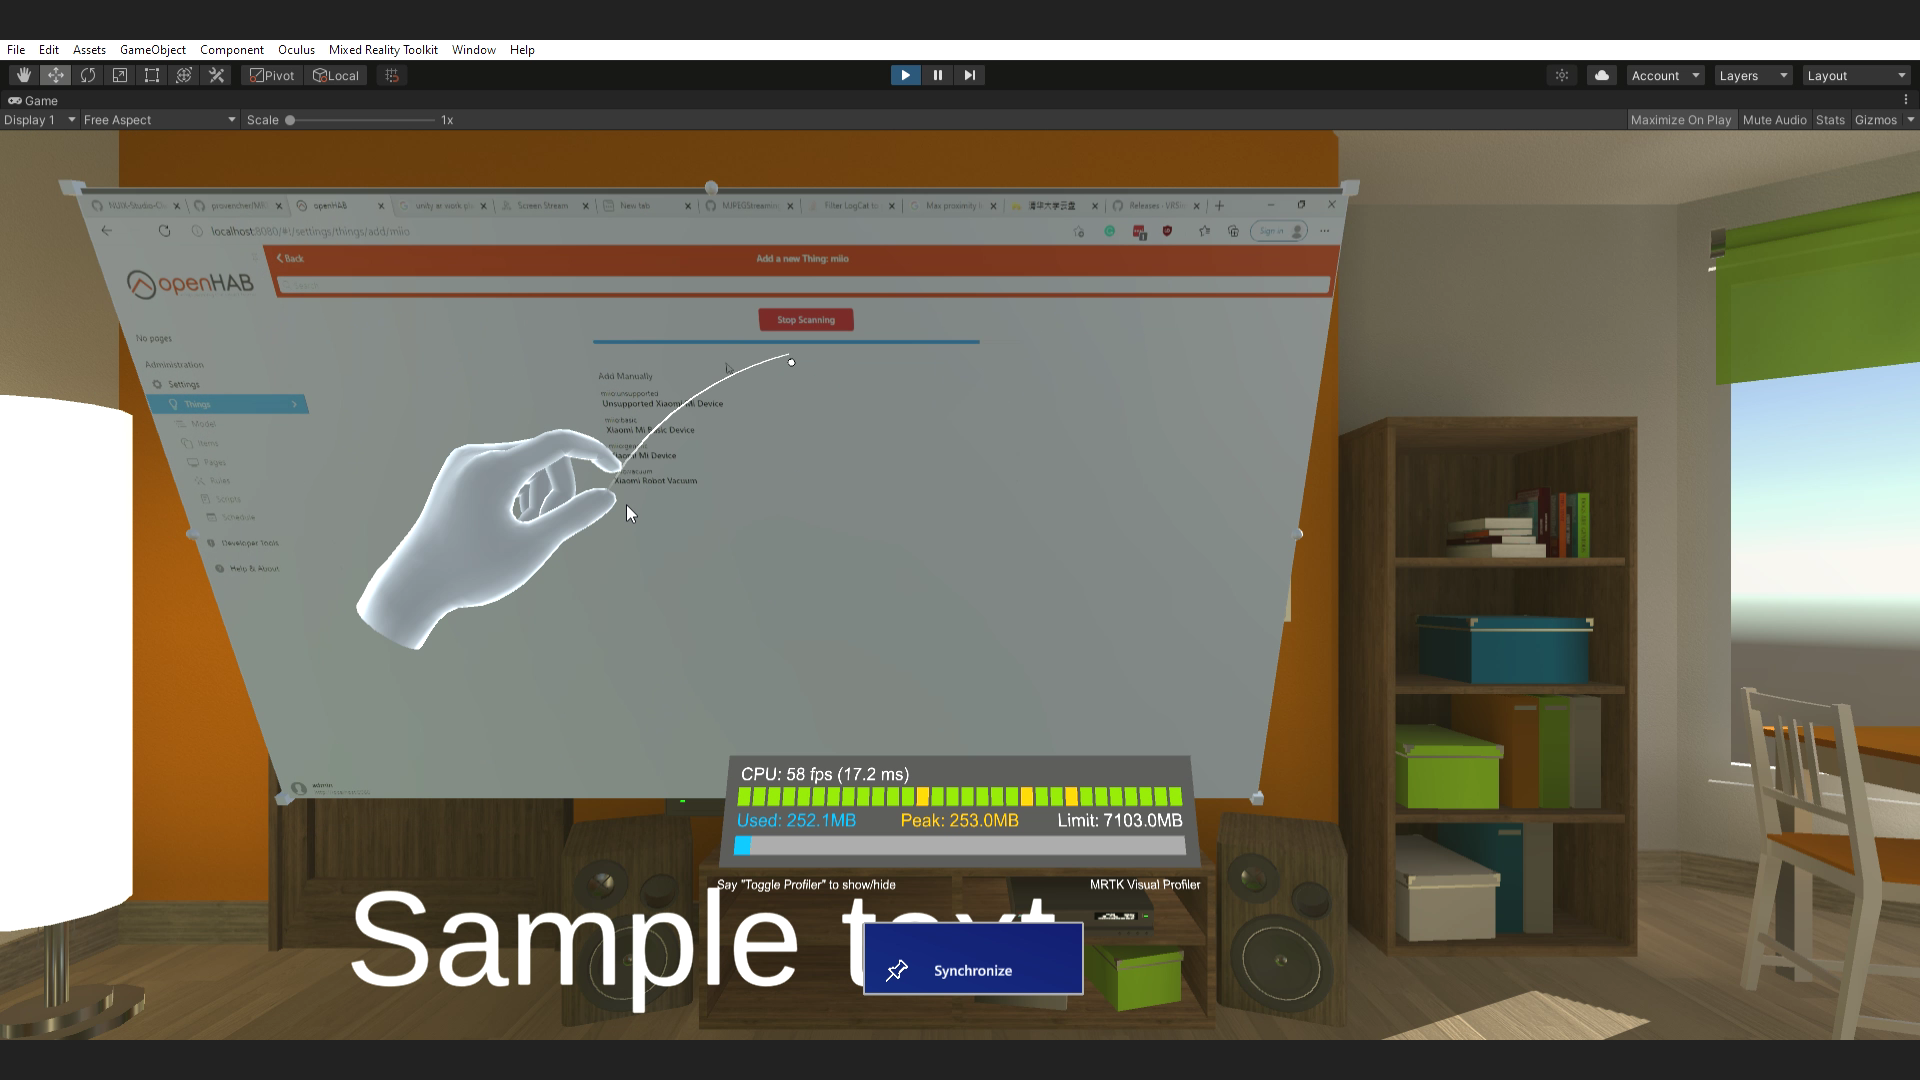
\includegraphics[width=0.45\linewidth]{figures/InputSimulation1.png}}
  \subcaptionbox{Pointing Gesture simulation\label{fig:InputSimulation-b}}
    {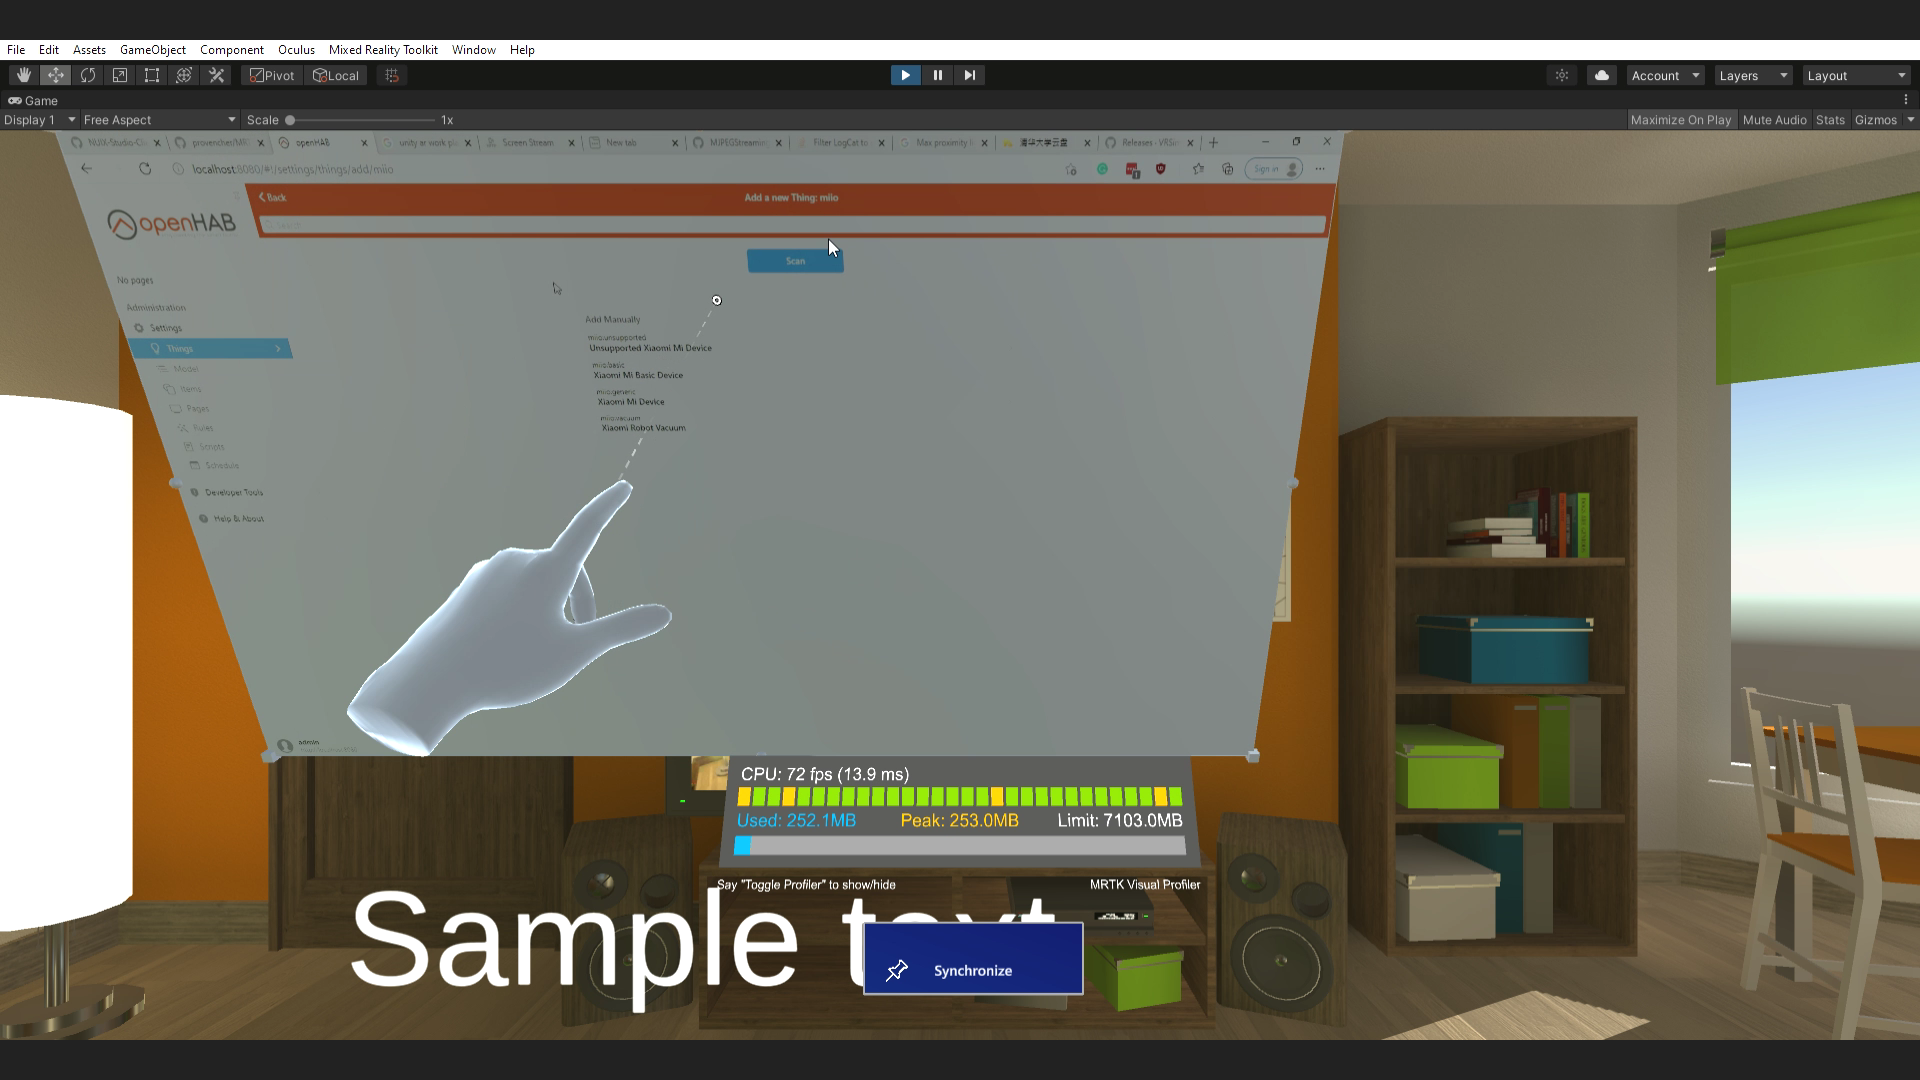
\includegraphics[width=0.45\linewidth]{figures/InputSimulation2.png}}
  \caption{Simulations of gestures on the UNIX-Studio App running on a PC.}
  \label{fig:InputSimulation-figure}
\end{figure}

In the final prototype (Figure~\ref{fig:FinalPrototype-figure}), code for the most of the items had been rewritten to support the new architecture defined in the previous chapters. 


\begin{figure}
  \centering
  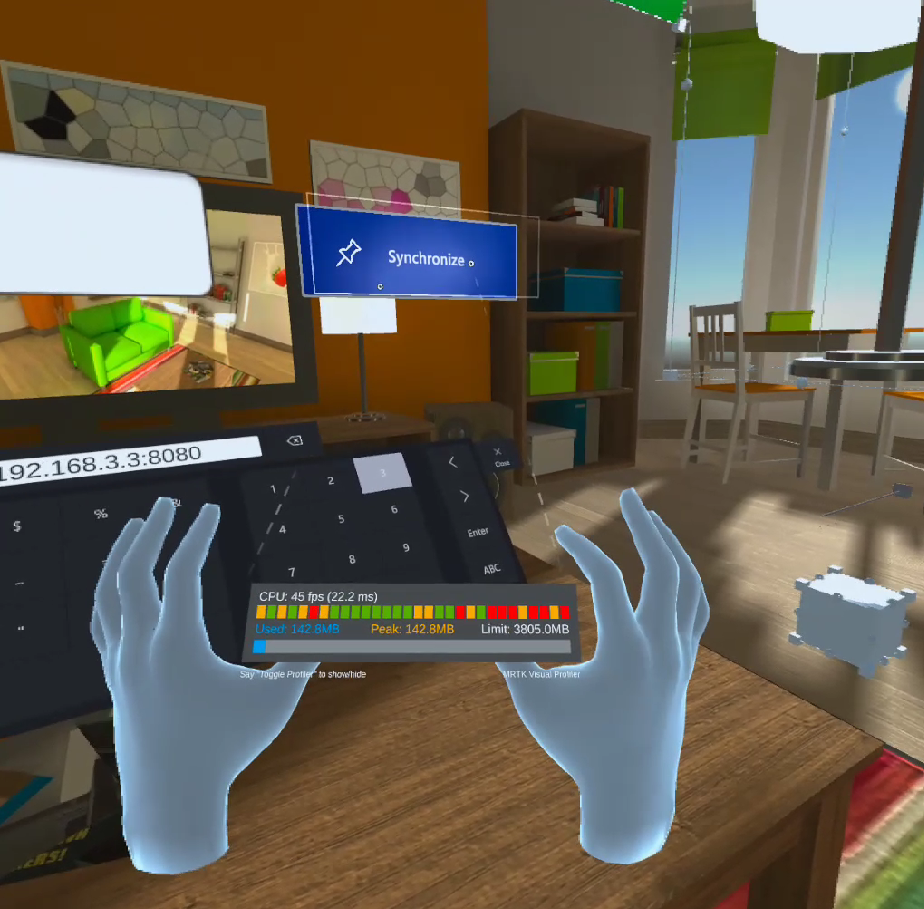
\includegraphics[width=0.6\linewidth]{figures/FinalPrototype.png}
  \caption{Screenshot of the final prototype of NUIX-Studio.}
  \label{fig:FinalPrototype-figure}
\end{figure}